\chapter{适应未知背景的可微分逆渲染方法}
\label{chap:method}

在将可微分渲染方法应用到3D人脸重建任务时,现有方法均未能充分利用可见性梯度。
而该梯度正是所有梯度中的主要分量,对模型与照片的精确对齐有着重要作用。
通常来说,计算正确的可见性梯度需要同时具有前景和背景的模型,而在自然环境照片中,由于背景多样,很难得到显式的背景模型。
本章主要针对该问题,提出一种适应未知背景的可微分渲染方法,能够利用可见性梯度来优化模型与照片的对齐。

\section{问题定义}

可微分渲染旨在从参数化的3D模型,如三角形面片,纹理贴图等,渲染得到2D图片,同时计算该渲染结果关于其输入参数的梯度。
然后可以优化渲染结果与照片间的误差,以期利用基于梯度的方法优化输入参数,从而改善渲染效果,使之更加接近现实。
其在3D人脸重建的相关任务中已有较广泛的应用。

然而现有方法存在一些不足:
现有可微分渲染技术大多是对整张图片估计梯度,即不区分前景和背景部分。
但是,在基于自然环境照片的人脸重建任务中,我们通常只有前景(即人脸)的3D模型,而没有背景的模型。
此时,现有方法选择忽略模型间相互遮挡产生的可见性梯度,而这会造成模型与照片的对齐不准确,如图\ref{fig:problem_a}所示。
另一方面,若对背景进行很粗糙的建模,例如假设为全黑,则错误的梯度会导致模型无法正确收敛,如图\ref{fig:problem_b}所示。

\begin{figure}
\centering
\begin{subfigure}[t]{0.45\textwidth}
    \centering
    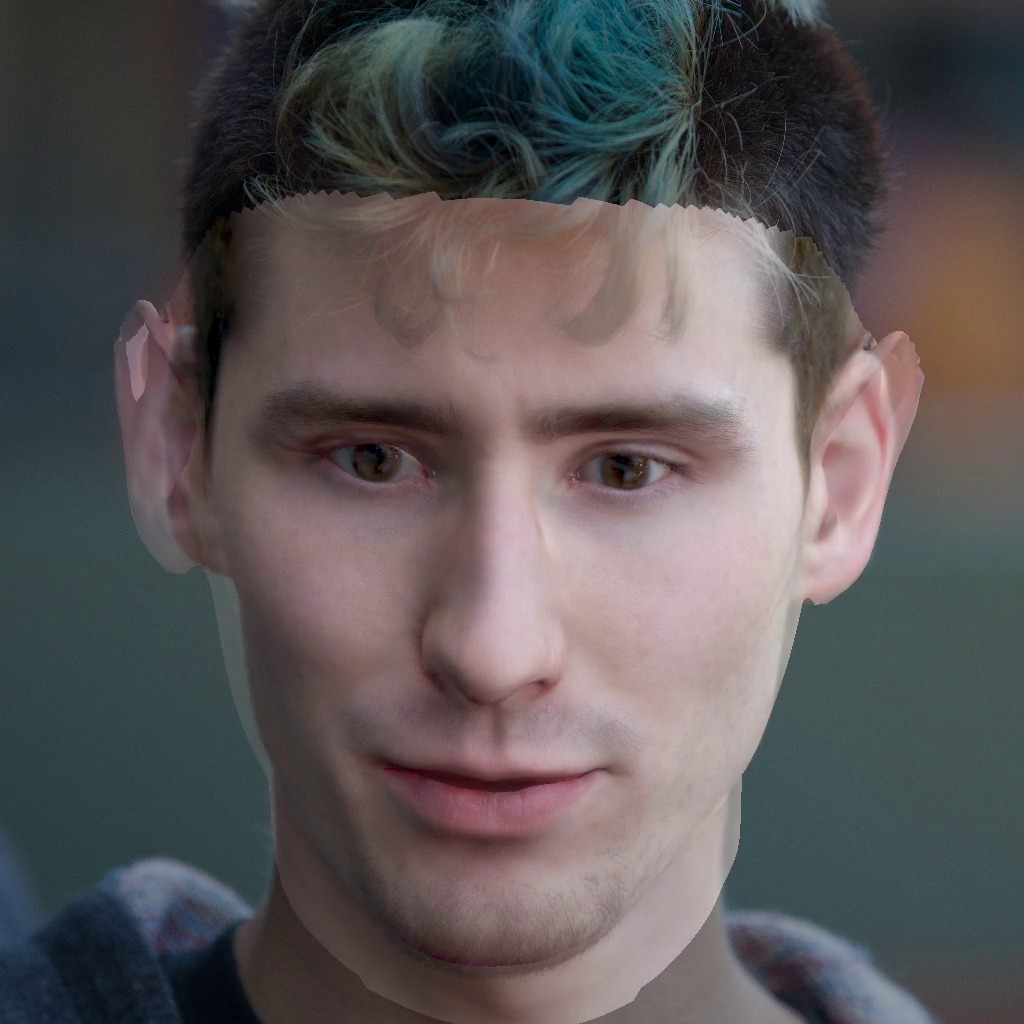
\includegraphics[width=\textwidth]{figures/black-bg_no-aa}
    \caption{忽略可见性梯度,模型与照片未准确对齐}
    \label{fig:problem_a}
\end{subfigure}
\begin{subfigure}[t]{0.45\textwidth}
    \centering
    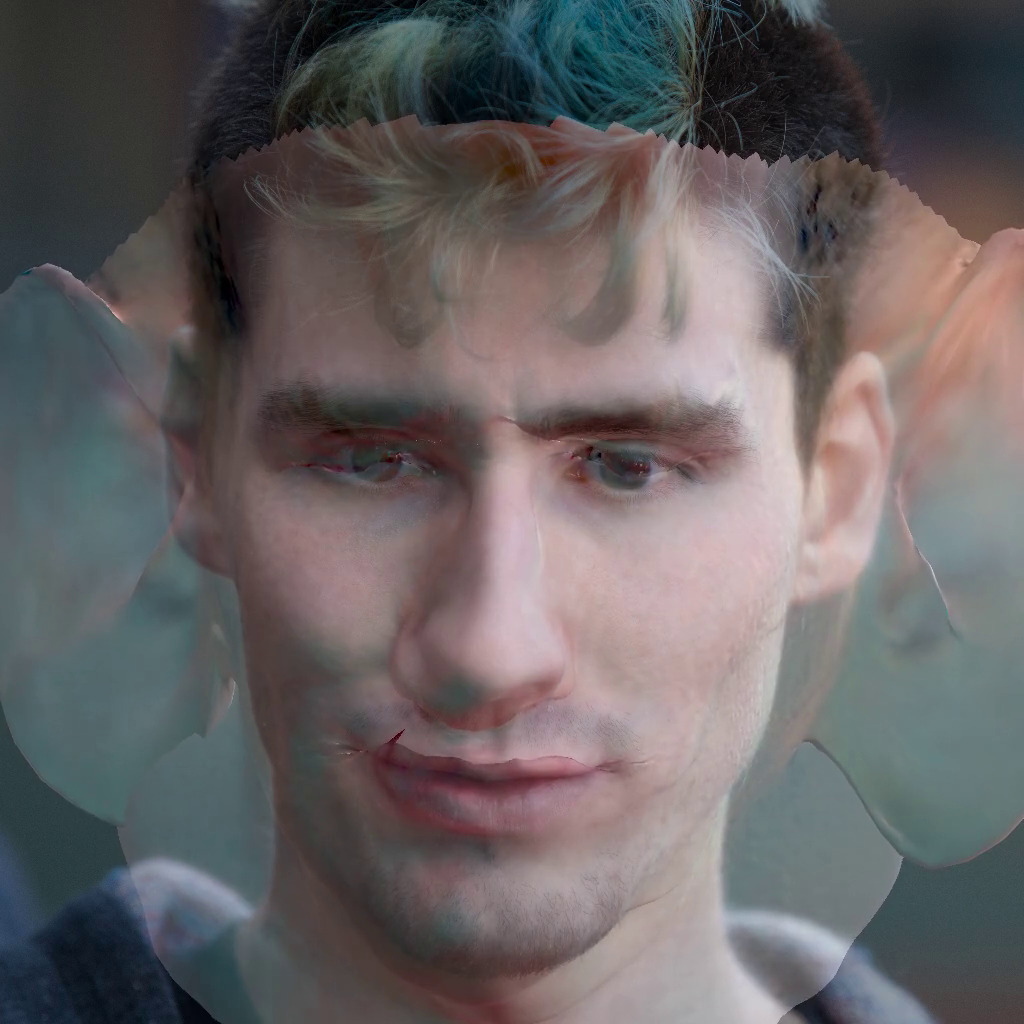
\includegraphics[width=\textwidth]{figures/black-bg}
    \caption{使用全黑代替背景模型,可见性梯度错误}
    \label{fig:problem_b}
\end{subfigure}
\caption[未知背景条件下可微分渲染优化结果]{
    未知背景条件下可微分渲染优化结果。
    示意图为目标照片和渲染结果以1:1 alpha混合后,再进行gammar校正得到。
}
\end{figure}

为绕过上述问题,现有方法通常:
使用多目立体等其他手段事先确定高精度的人脸几何形状,并在逆渲染优化过程中使几何形状保持不变\citep{RiviereGBGB20};
忽略可见性梯度,使用2D人脸关键点\citep{deep3d}、图像分割\citep{nvdiffrec}结果等辅助监督信息来补足这部分缺失的梯度。
但是,如果能够直接利用可见性梯度,可大大简化算法的流程,同时也能避免在前序步骤中引入额外的误差。

本节将设计一个简单的玩具实验来更直观地说明上述问题。
如图\ref{fig:problem}所示,我们使用一个简单的白色平面作为前景模型,用其拟合一个白色青色对半分割的场景。
该模型的参数是其横向的平移量,用平面边缘与横坐标轴的交点$a_x$表示。
该平面的边缘稍微倾斜,以突出可见性梯度的变化。
该平面的着色不受参数影响,始终固定为白色。
该例子中使用的损失函数为L1误差,即:
\begin{equation}
\mathcal{L} = \left\| \hat{\mathcal{I}} - \mathcal{I} \right\|_1
\text{。}
\label{eq:loss_l1}
\end{equation}

\begin{figure}
\centering
\import{build/figures}{problem.pgf}
\caption[在未知背景时计算可见性梯度困难]{
    在未知背景时计算可见性梯度困难。
    拟合目标和渲染结果左侧白色为前景,右侧为背景。
    前景模型为以红线为边界的白色平面。
    横坐标为前景模型的平移量。
    a)离散采样,不计算可见性梯度;
    b)使用不准确的黑色背景模型计算可见性梯度,模型无法收敛到期望位置;
    c)理想情况下,在完全已知背景时的可见性梯度,模型能准确收敛至梯度为0的点。
}
\label{fig:problem}
\end{figure}

其中,a)为离散采样的方式,也是目前大多人脸重建中使用的方法。
其渲染流程为:在每个像素的中点处采样,若其位于前景模型的覆盖范围内,则渲染为白色,否则渲染为背景。
由于采样过程是离散的,且$a_x$的改变并不会影响采样的模式,因此,渲染结果$\hat{\mathcal{I}}$关于$a_x$的梯度为0,其损失函数为阶梯函数。
即该损失函数完全无法以基于梯度的方式指导模型拟合。

另一方面,在没有准确背景模型的前提向,可见性梯度则难以被利用。
例如,在b)中,假设我们并不知道该场景的背景,因此直接假设其为全黑。
但在本例中这个假设显然是不准确的。
b)和c)的渲染方式与a)不同,其每个像素的颜色取决于前景模型覆盖该像素的面积的比例,并按面积比例线性混合前景和背景的颜色。
这使得处于前景边缘处的像素的颜色成为了关于$a_x$的连续函数,即产生了所谓的可见性梯度。
在此前提下,从图中可以观察到其损失函数呈递减的趋势,并未在期望的位置上形成极值。
因此,该梯度也无法引导模型收敛到期望的位置。

作为参考,c)展示了理想中,完全已知背景的情况下,可见性梯度的作用。
从图中可见,其损失函数在期望的位置上有一个明显的极值,且其周围的梯度将能很好地指导优化器,使模型收敛到该位置。

然而,在实际人脸重建的任务中,特别是从自然环境照片的重建中,背景可能是很复杂且难以建模的。
本章将探讨如何在这种情况下,如何利用可见性梯度以指导前景模型与目标照片对齐。

\section{面积归一化的像素损失函数}

在分析中,不妨先将目标照片$\hat{\mathcal{I}}$和渲染结果$\mathcal{I}$抽象为连续的颜色场$\mathbb{R}^2 \to \mathbb{R}^3$。
于是公式\ref{eq:loss_l1}中的原始L1损失函数可改写为:
\begin{equation}
\mathcal{L} = \iint_{\mathcal{A}} \left\| \hat{\mathcal{I}} - \mathcal{I} \right\|_1 \mathrm{d}\sigma +
\iint_{\mathcal{B}} \left\| \hat{\mathcal{I}} - \mathcal{I} \right\|_1 \mathrm{d}\sigma
\text{,}
\label{eq:loss_l1_area}
\end{equation}
其中,$\mathcal{A}$为渲染结果中前景模型覆盖的区域,$\mathcal{B}$为背景覆盖的区域。
由此我们可以对图\ref{fig:problem}b中的现象进一步地解释:
当前景模型的边界向右移动越过中点之后,由于不能很好地拟合背景,该损失函数的第一项开始上升,这是符合预期的。
但是,由于采用的背景模型不准确,背景部分也存在一定误差,且由于背景区域面积下降,损失函数的第二项将会下降。
这两项相互制衡,导致前景和背景模型“抢夺”处于交界处的像素。
若背景模型的误差足够大,以至于使用前景模型来拟合背景区域反而占优势,则会出现如b)中的现象:前景模型将在优化中不断抢占背景的区域,从而无法收敛到期望的位置。
在实际中这种情况是很有可能的,比如在3D人脸重建中,人脸的材质模型通常具有很高的自由度以拟合人脸的细节,这些自由度可能被误用于拟合背景。

为解决在未知背景下的逆渲染问题,本文提出了一种面积归一化的像素损失函数:
\begin{equation}
\mathcal{L}_n = \frac{\iint_{\mathcal{A}} \left\| \hat{\mathcal{I}} - \mathcal{I} \right\|_1 \mathrm{d}\sigma}
{\iint_{\mathcal{A}}\mathrm{d}\sigma}
-\alpha\iint_{\mathcal{A}}\mathrm{d}\sigma
\text{。}
\end{equation}
该损失函数仅在前景模型覆盖的区域内计算损失,因此不会受到背景模型的误差影响。
该函数第一项为单位前景区域面积内的平均误差,第二项鼓励更大的前景区域,$\alpha$为一个超参数。

\begin{figure}
\centering
\import{build/figures}{one_dim_loss.pgf}
\caption{面积归一化的像素损失函数在一维的作用分析}
\label{fig:one_dim_loss}
\end{figure}

为了更好地理解该损失函数的作用,本文将展示一个一维情况下的简单例子。
如图\ref{fig:one_dim_loss}a所示,假设拟合目标包含前景和背景,为阶跃函数;前景模型为定义在前景区域$\mathcal{A}=(0,\theta)$的常函数,$\theta$为模型参数:
\begin{align}
\mathcal{I}(x) &= \begin{cases}
    1   & x \leq 0.6 \\
    0.1 & x > 0.6
\end{cases}\\
\hat{\mathcal{I}}(x) &= 0.8 \quad x < \theta
\text{。}
\end{align}
在此定义下,我们可求出$\mathcal{L}_n(\theta)$中各项的解析表达式:
\begin{align}
\int_{\mathcal{A}} \left\| \hat{\mathcal{I}} - \mathcal{I} \right\|_1 \mathrm{d}\sigma
&= \int_0^{\theta} \left| \hat{\mathcal{I}}(x) - \mathcal{I}(x) \right| \mathrm{d}x \\
\int_{\mathcal{A}}\mathrm{d}\sigma &= \int_0^{\theta} \mathrm{d}x = \theta
\text{。}
\end{align}
其函数图像如图\ref{fig:one_dim_loss}b、c、d所示。
该函数第一项的分子为公式\ref{eq:loss_l1_area}中的第一项前景部分,显然该项是随着$\theta$单调递增的。
由于没有了背景部分的制衡,单独使用该项将导致模型收敛到一个很小的区域。
于是本文将该项以前景区域的面积进行归一化,即$\mathcal{L}_n$的第一项。
若该模型的拟合误差在前景区域内是均匀分布的,则该项将会是一个常数,不会引导模型减小面积。
而模型拟合背景区域的误差通常显著大于拟合前景,因此该项鼓励模型离开背景区域,从而减小平均误差。
而在当前景区域小于期望时,$\mathcal{L}_n$的第二项将会鼓励模型增大面积,准确对齐到目标的边界上。如图d)所示,$\mathcal{L}_n$在$\theta=0.6$处取得极值,此时模型的前景区域正好对齐了目标的边界。
同时,若有拟合误差在边缘处大于中心的情况,第二项也能提供一定的补偿。
直观地,若拟合目标具有清晰的边界,且在边界处模型拟合前景的误差小于拟合背景的误差,则存在一个$\alpha$,使模型能精确对齐到该边界上。

推广到二维的情况会稍微复杂,因为在二维下边界不止一个点,而边界的不同位置将会有不同情况。但根据以上分析,本章提出的损失函数最适用于以下场景:
\begin{enumerate*}
    \item 背景复杂且未知,但拟合目标具有清晰的边界;
    \item 在前景物体边界附近的拟合误差不显著高于中心区域;
    \item 在边界上,模型拟合前景的误差小于拟合背景的误差。
\end{enumerate*}
若在边界的个别区段上不能满足上述条件,则需要通过一定的平滑等正则化方法进行补偿。
常见的情况比如:
由于景深浅,照片中物体边缘有较大模糊;
或者在部分位置碰巧前景与背景颜色相似等。

\section{收缩\&扩展梯度}

本节将介绍如何将上一节提出的,定义在连续空间的损失函数应用于由离散的像素组成的图像上,并最终实现为收缩和扩展两项梯度的形式。

为了使损失函数成为关于渲染图像$\hat{\mathcal{I}}$的l连续函数,我们将图像渲染的过程定义为:
\begin{equation}
\hat{\mathcal{I}}(x,y;\theta) \to (\mathbf{c}, \sigma) \quad x,y \in \mathbb{Z}
\text{。}
\end{equation}
其中$x,y$为像素坐标,$\theta$为前景模型的参数,$\mathbf{c}\in\mathbb{R}^3$为着色后的像素颜色,且对模型覆盖区域外的像素没有定义,$\sigma\in[0,1]$为前景模型覆盖该像素的覆盖率,即该像素中被模型覆盖的面积占其总面积的比例。
$\mathbf{c}$的值取决于所选择的着色模型,因此在本章中不考虑其关于$\theta$的梯度。
自然地,对于处在模型内部的像素$\sigma=1$,而对于模型外部的像素$\sigma=0$,
仅当像素位于模型边界上时,$\frac{\partial\sigma}{\partial\theta}$才不为0,因此处于模型边界上的覆盖率$\sigma$是本节主要考虑的对象。
需要注意的是,准确地求出每个像素的$\sigma$运算量较大,后文第\ref{sec:method_discuss}节将介绍一种实现方式。

基于该定义,我们可以重新定义渲染图像与目标图像的距离为:
\begin{equation}
\left\|\hat{\mathcal{I}}(x,y;\theta) - \mathcal{I}(x,y)\right\| = \sigma\left\|\mathbf{c} - \mathcal{I}\right\|_1
\text{。}
\end{equation}
将该定义带入公式\ref{eq:loss}中,得到:

\section{实验结果}

\section{讨论}
\label{sec:method_discuss}

L1损失函数的必要性

模型裁减边缘的梯度处理

基于nvdiffrast\citep{nvdiffrast}的实现:
其可见性梯度的计算是稀疏的,
因此需要收缩扩展相互耦合;
手动放大可见性梯度。
